\documentclass[11pt]{article}

    \usepackage[breakable]{tcolorbox}
    \usepackage{parskip} % Stop auto-indenting (to mimic markdown behaviour)
    

    % Basic figure setup, for now with no caption control since it's done
    % automatically by Pandoc (which extracts ![](path) syntax from Markdown).
    \usepackage{graphicx}
    % Maintain compatibility with old templates. Remove in nbconvert 6.0
    \let\Oldincludegraphics\includegraphics
    % Ensure that by default, figures have no caption (until we provide a
    % proper Figure object with a Caption API and a way to capture that
    % in the conversion process - todo).
    \usepackage{caption}
    %\DeclareCaptionFormat{nocaption}{}
    %\captionsetup{format=nocaption,aboveskip=0pt,belowskip=0pt}

    \usepackage{float}
    \floatplacement{figure}{H} % forces figures to be placed at the correct location
    \usepackage{xcolor} % Allow colors to be defined
    \usepackage{enumerate} % Needed for markdown enumerations to work
    \usepackage{geometry} % Used to adjust the document margins
    \usepackage{amsmath} % Equations
    \usepackage{amssymb} % Equations
    \usepackage{textcomp} % defines textquotesingle
    % Hack from http://tex.stackexchange.com/a/47451/13684:
    \AtBeginDocument{%
        \def\PYZsq{\textquotesingle}% Upright quotes in Pygmentized code
    }
    \usepackage{upquote} % Upright quotes for verbatim code
    \usepackage{eurosym} % defines \euro

    \usepackage{iftex}
    \ifPDFTeX
        \usepackage[T1]{fontenc}
        \IfFileExists{alphabeta.sty}{
              \usepackage{alphabeta}
          }{
              \usepackage[mathletters]{ucs}
              \usepackage[utf8x]{inputenc}
          }
    \else
        \usepackage{fontspec}
        \usepackage{unicode-math}
    \fi

    \usepackage{fancyvrb} % verbatim replacement that allows latex
    \usepackage{grffile} % extends the file name processing of package graphics 
                         % to support a larger range
    \makeatletter % fix for old versions of grffile with XeLaTeX
    \@ifpackagelater{grffile}{2019/11/01}
    {
      % Do nothing on new versions
    }
    {
      \def\Gread@@xetex#1{%
        \IfFileExists{"\Gin@base".bb}%
        {\Gread@eps{\Gin@base.bb}}%
        {\Gread@@xetex@aux#1}%
      }
    }
    \makeatother
    \usepackage[Export]{adjustbox} % Used to constrain images to a maximum size
    \adjustboxset{max size={0.9\linewidth}{0.9\paperheight}}

    % The hyperref package gives us a pdf with properly built
    % internal navigation ('pdf bookmarks' for the table of contents,
    % internal cross-reference links, web links for URLs, etc.)
    \usepackage{hyperref}
    % The default LaTeX title has an obnoxious amount of whitespace. By default,
    % titling removes some of it. It also provides customization options.
    \usepackage{titling}
    \usepackage{longtable} % longtable support required by pandoc >1.10
    \usepackage{booktabs}  % table support for pandoc > 1.12.2
    \usepackage{array}     % table support for pandoc >= 2.11.3
    \usepackage{calc}      % table minipage width calculation for pandoc >= 2.11.1
    \usepackage[inline]{enumitem} % IRkernel/repr support (it uses the enumerate* environment)
    \usepackage[normalem]{ulem} % ulem is needed to support strikethroughs (\sout)
                                % normalem makes italics be italics, not underlines
    \usepackage{mathrsfs}
    \usepackage{listings}
    \definecolor{codegreen}{rgb}{0,0.6,0}
    \definecolor{codegray}{rgb}{0.5,0.5,0.5}
    \definecolor{codepurple}{rgb}{0.58,0,0.82}
    \definecolor{backcolour}{rgb}{0.95,0.95,0.92}
    
    \lstdefinestyle{mystyle}{
        backgroundcolor=\color{backcolour},   
        commentstyle=\color{codegreen},
        keywordstyle=\color{magenta},
        numberstyle=\tiny\color{codegray},
        stringstyle=\color{codepurple},
        basicstyle=\ttfamily\footnotesize,
        breakatwhitespace=false,         
        breaklines=true,                 
        captionpos=b,                    
        keepspaces=true,                 
        numbers=left,                    
        numbersep=5pt,                  
        showspaces=false,                
        showstringspaces=false,
        showtabs=false,                  
        tabsize=2
    }
    
    \lstset{style=mystyle}
    

    
    % Colors for the hyperref package
    \definecolor{urlcolor}{rgb}{0,.145,.698}
    \definecolor{linkcolor}{rgb}{.71,0.21,0.01}
    \definecolor{citecolor}{rgb}{.12,.54,.11}

    % ANSI colors
    \definecolor{ansi-black}{HTML}{3E424D}
    \definecolor{ansi-black-intense}{HTML}{282C36}
    \definecolor{ansi-red}{HTML}{E75C58}
    \definecolor{ansi-red-intense}{HTML}{B22B31}
    \definecolor{ansi-green}{HTML}{00A250}
    \definecolor{ansi-green-intense}{HTML}{007427}
    \definecolor{ansi-yellow}{HTML}{DDB62B}
    \definecolor{ansi-yellow-intense}{HTML}{B27D12}
    \definecolor{ansi-blue}{HTML}{208FFB}
    \definecolor{ansi-blue-intense}{HTML}{0065CA}
    \definecolor{ansi-magenta}{HTML}{D160C4}
    \definecolor{ansi-magenta-intense}{HTML}{A03196}
    \definecolor{ansi-cyan}{HTML}{60C6C8}
    \definecolor{ansi-cyan-intense}{HTML}{258F8F}
    \definecolor{ansi-white}{HTML}{C5C1B4}
    \definecolor{ansi-white-intense}{HTML}{A1A6B2}
    \definecolor{ansi-default-inverse-fg}{HTML}{FFFFFF}
    \definecolor{ansi-default-inverse-bg}{HTML}{000000}

    % common color for the border for error outputs.
    \definecolor{outerrorbackground}{HTML}{FFDFDF}

    % commands and environments needed by pandoc snippets
    % extracted from the output of `pandoc -s`
    \providecommand{\tightlist}{%
      \setlength{\itemsep}{0pt}\setlength{\parskip}{0pt}}
    \DefineVerbatimEnvironment{Highlighting}{Verbatim}{commandchars=\\\{\}}
    % Add ',fontsize=\small' for more characters per line
    \newenvironment{Shaded}{}{}
    \newcommand{\KeywordTok}[1]{\textcolor[rgb]{0.00,0.44,0.13}{\textbf{{#1}}}}
    \newcommand{\DataTypeTok}[1]{\textcolor[rgb]{0.56,0.13,0.00}{{#1}}}
    \newcommand{\DecValTok}[1]{\textcolor[rgb]{0.25,0.63,0.44}{{#1}}}
    \newcommand{\BaseNTok}[1]{\textcolor[rgb]{0.25,0.63,0.44}{{#1}}}
    \newcommand{\FloatTok}[1]{\textcolor[rgb]{0.25,0.63,0.44}{{#1}}}
    \newcommand{\CharTok}[1]{\textcolor[rgb]{0.25,0.44,0.63}{{#1}}}
    \newcommand{\StringTok}[1]{\textcolor[rgb]{0.25,0.44,0.63}{{#1}}}
    \newcommand{\CommentTok}[1]{\textcolor[rgb]{0.38,0.63,0.69}{\textit{{#1}}}}
    \newcommand{\OtherTok}[1]{\textcolor[rgb]{0.00,0.44,0.13}{{#1}}}
    \newcommand{\AlertTok}[1]{\textcolor[rgb]{1.00,0.00,0.00}{\textbf{{#1}}}}
    \newcommand{\FunctionTok}[1]{\textcolor[rgb]{0.02,0.16,0.49}{{#1}}}
    \newcommand{\RegionMarkerTok}[1]{{#1}}
    \newcommand{\ErrorTok}[1]{\textcolor[rgb]{1.00,0.00,0.00}{\textbf{{#1}}}}
    \newcommand{\NormalTok}[1]{{#1}}
    
    % Additional commands for more recent versions of Pandoc
    \newcommand{\ConstantTok}[1]{\textcolor[rgb]{0.53,0.00,0.00}{{#1}}}
    \newcommand{\SpecialCharTok}[1]{\textcolor[rgb]{0.25,0.44,0.63}{{#1}}}
    \newcommand{\VerbatimStringTok}[1]{\textcolor[rgb]{0.25,0.44,0.63}{{#1}}}
    \newcommand{\SpecialStringTok}[1]{\textcolor[rgb]{0.73,0.40,0.53}{{#1}}}
    \newcommand{\ImportTok}[1]{{#1}}
    \newcommand{\DocumentationTok}[1]{\textcolor[rgb]{0.73,0.13,0.13}{\textit{{#1}}}}
    \newcommand{\AnnotationTok}[1]{\textcolor[rgb]{0.38,0.63,0.69}{\textbf{\textit{{#1}}}}}
    \newcommand{\CommentVarTok}[1]{\textcolor[rgb]{0.38,0.63,0.69}{\textbf{\textit{{#1}}}}}
    \newcommand{\VariableTok}[1]{\textcolor[rgb]{0.10,0.09,0.49}{{#1}}}
    \newcommand{\ControlFlowTok}[1]{\textcolor[rgb]{0.00,0.44,0.13}{\textbf{{#1}}}}
    \newcommand{\OperatorTok}[1]{\textcolor[rgb]{0.40,0.40,0.40}{{#1}}}
    \newcommand{\BuiltInTok}[1]{{#1}}
    \newcommand{\ExtensionTok}[1]{{#1}}
    \newcommand{\PreprocessorTok}[1]{\textcolor[rgb]{0.74,0.48,0.00}{{#1}}}
    \newcommand{\AttributeTok}[1]{\textcolor[rgb]{0.49,0.56,0.16}{{#1}}}
    \newcommand{\InformationTok}[1]{\textcolor[rgb]{0.38,0.63,0.69}{\textbf{\textit{{#1}}}}}
    \newcommand{\WarningTok}[1]{\textcolor[rgb]{0.38,0.63,0.69}{\textbf{\textit{{#1}}}}}
    
    
    % Define a nice break command that doesn't care if a line doesn't already
    % exist.
    \def\br{\hspace*{\fill} \\* }
    % Math Jax compatibility definitions
    \def\gt{>}
    \def\lt{<}
    \let\Oldtex\TeX
    \let\Oldlatex\LaTeX
    \renewcommand{\TeX}{\textrm{\Oldtex}}
    \renewcommand{\LaTeX}{\textrm{\Oldlatex}}
    % Document parameters
    % Document title
    \title{PEC 3}
    
    
    
    
    
% Pygments definitions
\makeatletter
\def\PY@reset{\let\PY@it=\relax \let\PY@bf=\relax%
    \let\PY@ul=\relax \let\PY@tc=\relax%
    \let\PY@bc=\relax \let\PY@ff=\relax}
\def\PY@tok#1{\csname PY@tok@#1\endcsname}
\def\PY@toks#1+{\ifx\relax#1\empty\else%
    \PY@tok{#1}\expandafter\PY@toks\fi}
\def\PY@do#1{\PY@bc{\PY@tc{\PY@ul{%
    \PY@it{\PY@bf{\PY@ff{#1}}}}}}}
\def\PY#1#2{\PY@reset\PY@toks#1+\relax+\PY@do{#2}}

\@namedef{PY@tok@w}{\def\PY@tc##1{\textcolor[rgb]{0.73,0.73,0.73}{##1}}}
\@namedef{PY@tok@c}{\let\PY@it=\textit\def\PY@tc##1{\textcolor[rgb]{0.24,0.48,0.48}{##1}}}
\@namedef{PY@tok@cp}{\def\PY@tc##1{\textcolor[rgb]{0.61,0.40,0.00}{##1}}}
\@namedef{PY@tok@k}{\let\PY@bf=\textbf\def\PY@tc##1{\textcolor[rgb]{0.00,0.50,0.00}{##1}}}
\@namedef{PY@tok@kp}{\def\PY@tc##1{\textcolor[rgb]{0.00,0.50,0.00}{##1}}}
\@namedef{PY@tok@kt}{\def\PY@tc##1{\textcolor[rgb]{0.69,0.00,0.25}{##1}}}
\@namedef{PY@tok@o}{\def\PY@tc##1{\textcolor[rgb]{0.40,0.40,0.40}{##1}}}
\@namedef{PY@tok@ow}{\let\PY@bf=\textbf\def\PY@tc##1{\textcolor[rgb]{0.67,0.13,1.00}{##1}}}
\@namedef{PY@tok@nb}{\def\PY@tc##1{\textcolor[rgb]{0.00,0.50,0.00}{##1}}}
\@namedef{PY@tok@nf}{\def\PY@tc##1{\textcolor[rgb]{0.00,0.00,1.00}{##1}}}
\@namedef{PY@tok@nc}{\let\PY@bf=\textbf\def\PY@tc##1{\textcolor[rgb]{0.00,0.00,1.00}{##1}}}
\@namedef{PY@tok@nn}{\let\PY@bf=\textbf\def\PY@tc##1{\textcolor[rgb]{0.00,0.00,1.00}{##1}}}
\@namedef{PY@tok@ne}{\let\PY@bf=\textbf\def\PY@tc##1{\textcolor[rgb]{0.80,0.25,0.22}{##1}}}
\@namedef{PY@tok@nv}{\def\PY@tc##1{\textcolor[rgb]{0.10,0.09,0.49}{##1}}}
\@namedef{PY@tok@no}{\def\PY@tc##1{\textcolor[rgb]{0.53,0.00,0.00}{##1}}}
\@namedef{PY@tok@nl}{\def\PY@tc##1{\textcolor[rgb]{0.46,0.46,0.00}{##1}}}
\@namedef{PY@tok@ni}{\let\PY@bf=\textbf\def\PY@tc##1{\textcolor[rgb]{0.44,0.44,0.44}{##1}}}
\@namedef{PY@tok@na}{\def\PY@tc##1{\textcolor[rgb]{0.41,0.47,0.13}{##1}}}
\@namedef{PY@tok@nt}{\let\PY@bf=\textbf\def\PY@tc##1{\textcolor[rgb]{0.00,0.50,0.00}{##1}}}
\@namedef{PY@tok@nd}{\def\PY@tc##1{\textcolor[rgb]{0.67,0.13,1.00}{##1}}}
\@namedef{PY@tok@s}{\def\PY@tc##1{\textcolor[rgb]{0.73,0.13,0.13}{##1}}}
\@namedef{PY@tok@sd}{\let\PY@it=\textit\def\PY@tc##1{\textcolor[rgb]{0.73,0.13,0.13}{##1}}}
\@namedef{PY@tok@si}{\let\PY@bf=\textbf\def\PY@tc##1{\textcolor[rgb]{0.64,0.35,0.47}{##1}}}
\@namedef{PY@tok@se}{\let\PY@bf=\textbf\def\PY@tc##1{\textcolor[rgb]{0.67,0.36,0.12}{##1}}}
\@namedef{PY@tok@sr}{\def\PY@tc##1{\textcolor[rgb]{0.64,0.35,0.47}{##1}}}
\@namedef{PY@tok@ss}{\def\PY@tc##1{\textcolor[rgb]{0.10,0.09,0.49}{##1}}}
\@namedef{PY@tok@sx}{\def\PY@tc##1{\textcolor[rgb]{0.00,0.50,0.00}{##1}}}
\@namedef{PY@tok@m}{\def\PY@tc##1{\textcolor[rgb]{0.40,0.40,0.40}{##1}}}
\@namedef{PY@tok@gh}{\let\PY@bf=\textbf\def\PY@tc##1{\textcolor[rgb]{0.00,0.00,0.50}{##1}}}
\@namedef{PY@tok@gu}{\let\PY@bf=\textbf\def\PY@tc##1{\textcolor[rgb]{0.50,0.00,0.50}{##1}}}
\@namedef{PY@tok@gd}{\def\PY@tc##1{\textcolor[rgb]{0.63,0.00,0.00}{##1}}}
\@namedef{PY@tok@gi}{\def\PY@tc##1{\textcolor[rgb]{0.00,0.52,0.00}{##1}}}
\@namedef{PY@tok@gr}{\def\PY@tc##1{\textcolor[rgb]{0.89,0.00,0.00}{##1}}}
\@namedef{PY@tok@ge}{\let\PY@it=\textit}
\@namedef{PY@tok@gs}{\let\PY@bf=\textbf}
\@namedef{PY@tok@gp}{\let\PY@bf=\textbf\def\PY@tc##1{\textcolor[rgb]{0.00,0.00,0.50}{##1}}}
\@namedef{PY@tok@go}{\def\PY@tc##1{\textcolor[rgb]{0.44,0.44,0.44}{##1}}}
\@namedef{PY@tok@gt}{\def\PY@tc##1{\textcolor[rgb]{0.00,0.27,0.87}{##1}}}
\@namedef{PY@tok@err}{\def\PY@bc##1{{\setlength{\fboxsep}{\string -\fboxrule}\fcolorbox[rgb]{1.00,0.00,0.00}{1,1,1}{\strut ##1}}}}
\@namedef{PY@tok@kc}{\let\PY@bf=\textbf\def\PY@tc##1{\textcolor[rgb]{0.00,0.50,0.00}{##1}}}
\@namedef{PY@tok@kd}{\let\PY@bf=\textbf\def\PY@tc##1{\textcolor[rgb]{0.00,0.50,0.00}{##1}}}
\@namedef{PY@tok@kn}{\let\PY@bf=\textbf\def\PY@tc##1{\textcolor[rgb]{0.00,0.50,0.00}{##1}}}
\@namedef{PY@tok@kr}{\let\PY@bf=\textbf\def\PY@tc##1{\textcolor[rgb]{0.00,0.50,0.00}{##1}}}
\@namedef{PY@tok@bp}{\def\PY@tc##1{\textcolor[rgb]{0.00,0.50,0.00}{##1}}}
\@namedef{PY@tok@fm}{\def\PY@tc##1{\textcolor[rgb]{0.00,0.00,1.00}{##1}}}
\@namedef{PY@tok@vc}{\def\PY@tc##1{\textcolor[rgb]{0.10,0.09,0.49}{##1}}}
\@namedef{PY@tok@vg}{\def\PY@tc##1{\textcolor[rgb]{0.10,0.09,0.49}{##1}}}
\@namedef{PY@tok@vi}{\def\PY@tc##1{\textcolor[rgb]{0.10,0.09,0.49}{##1}}}
\@namedef{PY@tok@vm}{\def\PY@tc##1{\textcolor[rgb]{0.10,0.09,0.49}{##1}}}
\@namedef{PY@tok@sa}{\def\PY@tc##1{\textcolor[rgb]{0.73,0.13,0.13}{##1}}}
\@namedef{PY@tok@sb}{\def\PY@tc##1{\textcolor[rgb]{0.73,0.13,0.13}{##1}}}
\@namedef{PY@tok@sc}{\def\PY@tc##1{\textcolor[rgb]{0.73,0.13,0.13}{##1}}}
\@namedef{PY@tok@dl}{\def\PY@tc##1{\textcolor[rgb]{0.73,0.13,0.13}{##1}}}
\@namedef{PY@tok@s2}{\def\PY@tc##1{\textcolor[rgb]{0.73,0.13,0.13}{##1}}}
\@namedef{PY@tok@sh}{\def\PY@tc##1{\textcolor[rgb]{0.73,0.13,0.13}{##1}}}
\@namedef{PY@tok@s1}{\def\PY@tc##1{\textcolor[rgb]{0.73,0.13,0.13}{##1}}}
\@namedef{PY@tok@mb}{\def\PY@tc##1{\textcolor[rgb]{0.40,0.40,0.40}{##1}}}
\@namedef{PY@tok@mf}{\def\PY@tc##1{\textcolor[rgb]{0.40,0.40,0.40}{##1}}}
\@namedef{PY@tok@mh}{\def\PY@tc##1{\textcolor[rgb]{0.40,0.40,0.40}{##1}}}
\@namedef{PY@tok@mi}{\def\PY@tc##1{\textcolor[rgb]{0.40,0.40,0.40}{##1}}}
\@namedef{PY@tok@il}{\def\PY@tc##1{\textcolor[rgb]{0.40,0.40,0.40}{##1}}}
\@namedef{PY@tok@mo}{\def\PY@tc##1{\textcolor[rgb]{0.40,0.40,0.40}{##1}}}
\@namedef{PY@tok@ch}{\let\PY@it=\textit\def\PY@tc##1{\textcolor[rgb]{0.24,0.48,0.48}{##1}}}
\@namedef{PY@tok@cm}{\let\PY@it=\textit\def\PY@tc##1{\textcolor[rgb]{0.24,0.48,0.48}{##1}}}
\@namedef{PY@tok@cpf}{\let\PY@it=\textit\def\PY@tc##1{\textcolor[rgb]{0.24,0.48,0.48}{##1}}}
\@namedef{PY@tok@c1}{\let\PY@it=\textit\def\PY@tc##1{\textcolor[rgb]{0.24,0.48,0.48}{##1}}}
\@namedef{PY@tok@cs}{\let\PY@it=\textit\def\PY@tc##1{\textcolor[rgb]{0.24,0.48,0.48}{##1}}}

\def\PYZbs{\char`\\}
\def\PYZus{\char`\_}
\def\PYZob{\char`\{}
\def\PYZcb{\char`\}}
\def\PYZca{\char`\^}
\def\PYZam{\char`\&}
\def\PYZlt{\char`\<}
\def\PYZgt{\char`\>}
\def\PYZsh{\char`\#}
\def\PYZpc{\char`\%}
\def\PYZdl{\char`\$}
\def\PYZhy{\char`\-}
\def\PYZsq{\char`\'}
\def\PYZdq{\char`\"}
\def\PYZti{\char`\~}
% for compatibility with earlier versions
\def\PYZat{@}
\def\PYZlb{[}
\def\PYZrb{]}
\makeatother


    % For linebreaks inside Verbatim environment from package fancyvrb. 
    \makeatletter
        \newbox\Wrappedcontinuationbox 
        \newbox\Wrappedvisiblespacebox 
        \newcommand*\Wrappedvisiblespace {\textcolor{red}{\textvisiblespace}} 
        \newcommand*\Wrappedcontinuationsymbol {\textcolor{red}{\llap{\tiny$\m@th\hookrightarrow$}}} 
        \newcommand*\Wrappedcontinuationindent {3ex } 
        \newcommand*\Wrappedafterbreak {\kern\Wrappedcontinuationindent\copy\Wrappedcontinuationbox} 
        % Take advantage of the already applied Pygments mark-up to insert 
        % potential linebreaks for TeX processing. 
        %        {, <, #, %, $, ' and ": go to next line. 
        %        _, }, ^, &, >, - and ~: stay at end of broken line. 
        % Use of \textquotesingle for straight quote. 
        \newcommand*\Wrappedbreaksatspecials {% 
            \def\PYGZus{\discretionary{\char`\_}{\Wrappedafterbreak}{\char`\_}}% 
            \def\PYGZob{\discretionary{}{\Wrappedafterbreak\char`\{}{\char`\{}}% 
            \def\PYGZcb{\discretionary{\char`\}}{\Wrappedafterbreak}{\char`\}}}% 
            \def\PYGZca{\discretionary{\char`\^}{\Wrappedafterbreak}{\char`\^}}% 
            \def\PYGZam{\discretionary{\char`\&}{\Wrappedafterbreak}{\char`\&}}% 
            \def\PYGZlt{\discretionary{}{\Wrappedafterbreak\char`\<}{\char`\<}}% 
            \def\PYGZgt{\discretionary{\char`\>}{\Wrappedafterbreak}{\char`\>}}% 
            \def\PYGZsh{\discretionary{}{\Wrappedafterbreak\char`\#}{\char`\#}}% 
            \def\PYGZpc{\discretionary{}{\Wrappedafterbreak\char`\%}{\char`\%}}% 
            \def\PYGZdl{\discretionary{}{\Wrappedafterbreak\char`\$}{\char`\$}}% 
            \def\PYGZhy{\discretionary{\char`\-}{\Wrappedafterbreak}{\char`\-}}% 
            \def\PYGZsq{\discretionary{}{\Wrappedafterbreak\textquotesingle}{\textquotesingle}}% 
            \def\PYGZdq{\discretionary{}{\Wrappedafterbreak\char`\"}{\char`\"}}% 
            \def\PYGZti{\discretionary{\char`\~}{\Wrappedafterbreak}{\char`\~}}% 
        } 
        % Some characters . , ; ? ! / are not pygmentized. 
        % This macro makes them "active" and they will insert potential linebreaks 
        \newcommand*\Wrappedbreaksatpunct {% 
            \lccode`\~`\.\lowercase{\def~}{\discretionary{\hbox{\char`\.}}{\Wrappedafterbreak}{\hbox{\char`\.}}}% 
            \lccode`\~`\,\lowercase{\def~}{\discretionary{\hbox{\char`\,}}{\Wrappedafterbreak}{\hbox{\char`\,}}}% 
            \lccode`\~`\;\lowercase{\def~}{\discretionary{\hbox{\char`\;}}{\Wrappedafterbreak}{\hbox{\char`\;}}}% 
            \lccode`\~`\:\lowercase{\def~}{\discretionary{\hbox{\char`\:}}{\Wrappedafterbreak}{\hbox{\char`\:}}}% 
            \lccode`\~`\?\lowercase{\def~}{\discretionary{\hbox{\char`\?}}{\Wrappedafterbreak}{\hbox{\char`\?}}}% 
            \lccode`\~`\!\lowercase{\def~}{\discretionary{\hbox{\char`\!}}{\Wrappedafterbreak}{\hbox{\char`\!}}}% 
            \lccode`\~`\/\lowercase{\def~}{\discretionary{\hbox{\char`\/}}{\Wrappedafterbreak}{\hbox{\char`\/}}}% 
            \catcode`\.\active
            \catcode`\,\active 
            \catcode`\;\active
            \catcode`\:\active
            \catcode`\?\active
            \catcode`\!\active
            \catcode`\/\active 
            \lccode`\~`\~ 	
        }
    \makeatother

    \let\OriginalVerbatim=\Verbatim
    \makeatletter
    \renewcommand{\Verbatim}[1][1]{%
        %\parskip\z@skip
        \sbox\Wrappedcontinuationbox {\Wrappedcontinuationsymbol}%
        \sbox\Wrappedvisiblespacebox {\FV@SetupFont\Wrappedvisiblespace}%
        \def\FancyVerbFormatLine ##1{\hsize\linewidth
            \vtop{\raggedright\hyphenpenalty\z@\exhyphenpenalty\z@
                \doublehyphendemerits\z@\finalhyphendemerits\z@
                \strut ##1\strut}%
        }%
        % If the linebreak is at a space, the latter will be displayed as visible
        % space at end of first line, and a continuation symbol starts next line.
        % Stretch/shrink are however usually zero for typewriter font.
        \def\FV@Space {%
            \nobreak\hskip\z@ plus\fontdimen3\font minus\fontdimen4\font
            \discretionary{\copy\Wrappedvisiblespacebox}{\Wrappedafterbreak}
            {\kern\fontdimen2\font}%
        }%
        
        % Allow breaks at special characters using \PYG... macros.
        \Wrappedbreaksatspecials
        % Breaks at punctuation characters . , ; ? ! and / need catcode=\active 	
        \OriginalVerbatim[#1,codes*=\Wrappedbreaksatpunct]%
    }
    \makeatother

    % Exact colors from NB
    \definecolor{incolor}{HTML}{303F9F}
    \definecolor{outcolor}{HTML}{D84315}
    \definecolor{cellborder}{HTML}{CFCFCF}
    \definecolor{cellbackground}{HTML}{F7F7F7}
    
    % prompt
    \makeatletter
    \newcommand{\boxspacing}{\kern\kvtcb@left@rule\kern\kvtcb@boxsep}
    \makeatother
    \newcommand{\prompt}[4]{
        {\ttfamily\llap{{\color{#2}[#3]:\hspace{3pt}#4}}\vspace{-\baselineskip}}
    }
    

    
    % Prevent overflowing lines due to hard-to-break entities
    \sloppy 
    % Setup hyperref package
    \hypersetup{
      breaklinks=true,  % so long urls are correctly broken across lines
      colorlinks=true,
      urlcolor=urlcolor,
      linkcolor=linkcolor,
      citecolor=citecolor,
    }
    % Slightly bigger margins than the latex defaults
    
    \geometry{verbose,tmargin=1in,bmargin=1in,lmargin=1in,rmargin=1in}
    
    

\begin{document}
    \author{Pablo Riutort Grande}
    \maketitle
    
M0.534 - Chaotic Dynamical Systems

Master's Degree in Computational and Mathematical Engineering 

\hypertarget{1}{%
\section{}\label{1}}
    Suppose $f(z)$ has a fixed point at $z_0$. Then $z_0$ is \cite{chaos}:
    \begin{enumerate}
        \item Attracting if $\lvert f'(z_0) \rvert < 1$
        \item Repelling if $\lvert f'(z_0) \rvert > 1$
        \item Neutral if $\lvert f'(z_0) \rvert = 1$
    \end{enumerate}

    Plot the Dynamical Plane (Julia and Fatou sets) of $Q_c(z) = z^2+c$ for the following values of $c$.
\begin{enumerate}[label=(\alph{*})]
    \item $c_0 = -\frac{1}{2} - \frac{1}{10}i$. [Fig.\ref{fig:1a}]. Prove that $Q_{c_0}$ has an attracting fixed point.\\
    To prove that $Q_{c_0}(z)=z^2+c_0$ has an attrracting fixed point, we need to find a value of $z$ such that $Q_{c_0}(z) = z$ and the derivative of $Q_{c_0}$ evaluated at that point is $< 1$.
    \begin{equation}
        \begin{split}
        z^2 + c_0 = z \\
        z^2 + -z + c_0 = 0 \\
        z=\frac{-\left(-1\right)\pm\sqrt{-1^2-4\left(1\right)\left(c_0\right)}}{2}\\
        z=\frac{1\pm\sqrt{1-4\left(-\frac{1}{2} - \frac{1}{10}i\right)}}{2}\\
        z=\frac{1\pm\sqrt{1+2+\left(\frac{4}{10}i\right)}}{2}\\
        z=\frac{1\pm\sqrt{3+\left(\frac{2}{5}i\right)}}{2}\\
        z_1=\frac{1-\sqrt{3+\left(\frac{2}{5}i\right)}}{2}\\
        z_2=\frac{1+\sqrt{3+\left(\frac{2}{5}i\right)}}{2}\\
        \end{split}
    \end{equation}
    \begin{equation}
        \begin{split}
            Q_{c_0}'(z) = 2z\\
            Q_{c_0}'(z_1) = 2 \left(\frac{1-\sqrt{3+\left(\frac{2}{5}i\right)}}{2}\right)\\
            Q_{c_0}'(z_1) = 1-\sqrt{3+\left(\frac{2}{5}i\right)}\\
            Q_{c_0}'(z_1) = |-0.7358 - 0.1152 i| < 0
        \end{split}
    \end{equation}
    Hence $z_1$ is an attracting fixed point.
    \item $c_1 = \frac{1}{2}i$. [Fig.\ref{fig:1b}]. Prove that the $Q_{c_1}$ has an attracting fixed point.\\
    To prove that $Q_{c_1}(z)=z^2+c_1$ has an attrracting fixed point, we need to find a value of $z$ such that $Q_{c_1}(z) = z$ and the derivative of $Q_{c_1}$ evaluated at that point is $< 1$.
    \begin{equation}
        \begin{split}
        z^2 + c_1 = z \\
        z^2 + -z + c_1 = 0 \\
        z=\frac{-\left(-1\right)\pm\sqrt{-1^2-4\left(1\right)\left(c_1\right)}}{2}\\
        z=\frac{1\pm\sqrt{1-4\left(\frac{1}{2}i\right)}}{2}\\
        z=\frac{1\pm\sqrt{1-2i}}{2}\\
        z_1=\frac{1-\sqrt{1-2i}}{2}\\
        z_2=\frac{1+\sqrt{1-2i}}{2}\\
        \end{split}
    \end{equation}
    \begin{equation}
        \begin{split}
            Q_{c_1}'(z) = 2z\\
            Q_{c_1}'(z_1) = 2 \left(\frac{1-\sqrt{1-2i}}{2}\right)\\
            Q_{c_1}'(z_1) = 1-\sqrt{1-2i}\\
            Q_{c_1}'(z_1) = |-0.272 + 0.786i| < 0
        \end{split}
    \end{equation}
    Hence $z_1$ is an attracting fixed point.
    \item $c_2 = -1$. [Fig.\ref{fig:1c}]. Prove that the $Q_{c_2}$ has an attracting cycle of period two.
    To prove that $Q_{c_2}$​ has an attracting cycle of period two where $c_2 = -1$ we need to show the existence of two distinct points $z_1$, $z_2$ such that $Q_{c_2}(z_1) = z_2$ and $Q_{c_2}(z_2) = z_1$.\\
    We can start by evaluating $Q_{c_2}(z_1)$ on $c_2$:
    \begin{equation}
        \begin{split}
            Q_{c_2}(z_1) = z^2_1 - 1\\
            Q_{c_2}(z_1) = (-1)^2 - 1\\
            Q_{c_2}(z_1) = 0
        \end{split}
    \end{equation}

    Now we can proceed by substituing the value of $z_2$ by $z_1$ in:
    \begin{equation}
        \begin{split}
            Q_{c_2}(z_2) = z^2_2 - 1\\
            Q_{c_2}(z_2) = (0)^2 - 1\\
            Q_{c_2}(z_2) = -1
        \end{split}
    \end{equation}

    This shows that $Q_{c_2}(z_1) = z_2$ and $Q_{c_2}(z_2) = z_1$ and so there is a cycle of two.\\
    To see if this cycle is attracting we consider $z_1$ as a fixed point for $Q^2_{c_2}(z)$. We make use of the chain rule
    to compute $(Q^2_{c_2})'(z_1)$ \cite{chaos}:
    \begin{equation}\label{eq:chain}
        \begin{split}
            (Q^2_{c_2})'(z_1) = Q_{c_2}'(Q_{c_2}(z_1))Q_{c_2}'(z_1) = Q_{c_2}'(z_2)Q_{c_2}'(z_1) = 2(-1) 2(0) = 0 < 1.
        \end{split}
    \end{equation}
    Which means the 2-cycle is attracting.

     \item $c_3 = \frac{1}{4}$. [Fig.\ref{fig:1d}]. Prove that the $Q_{c_3}$ has a neutral fixed point.\\
    To prove that $Q_{c_3}(z)=z^2+\frac{1}{4}$ has a neutral fixed point, we need to find a value of $z$ such that $Q_{c_3}(z) = z$ and the derivative of $Q_{c_3}$ evaluated at that point is equal to 1.
    \begin{equation}
        \begin{split}
            z^2 + \frac{1}{4} = z \\
            z^2 -z + \frac{1}{4} = 0 \\
            \left(z - \frac{1}{2}\right)^2 = 0 \\
            z - \frac{1}{2} = 0 \\
            z = \frac{1}{2} \\
        \end{split}
    \end{equation}
    We now have a fixed point at $z = \frac{1}{2}$, let's evaluate the derivative of $Q_{c_3}$ at that point
    \begin{equation}
        \begin{split}
            Q_{c_3}'\left(z\right) = 2z \\
            Q_{c_3}'\left(\frac{1}{2}\right) = 2 \left(\frac{1}{2}\right) = 1\\
        \end{split}
    \end{equation}
    Then, $z = \frac{1}{2}$ is a neutral fixed point.

    \item $c_4 = -\frac{3}{4}$. [Fig.\ref{fig:1e}]. Prove that the $Q_{c_4}$ has a neutral cycle of period two.\\
    \begin{equation}
        \begin{split}
            Q_{c_4}(z_1) = z^2_1 - \frac{3}{4}\\
            Q_{c_4}(z_1) = z^2 - \frac{3}{4} = z\\
            Q_{c_4}(z_1) = z^2 - z - \frac{3}{4} = 0\\
            z_{1_a} = -\frac{1}{2} \\ z_{1_b} = \frac{3}{2}
        \end{split}
    \end{equation}
    \begin{equation}
        \begin{split}
        z_2 = (z_1)^2 - \frac{3}{4}
        \end{split}
    \end{equation}
    \begin{equation}
        \begin{split}
            Q_{c_4}\left(-\frac{1}{2}\right) = \left(-\frac{1}{2}\right)^2 - \frac{3}{4} = \frac{1}{4} - \frac{3}{4} = -\frac{2}{4} = - \frac{1}{2} = z_{1_a}\\
            Q_{c_4}\left(\frac{3}{2}\right) = \left(\frac{3}{2}\right)^2 - \frac{3}{4} = \frac{9}{4} - \frac{3}{4} = \frac{6}{4} = \frac{3}{2} = z_{1_b}
        \end{split}
    \end{equation}
    This shows that $Q_{c_4}(z_1) = z_2$ and $Q_{c_4}(z_2) = z_1$ and so there is a cycle of two.\\
    Similarly as in \ref{eq:chain} we can make use of the chain rule to observe its behaviour in $z_{1_a}$:
    \begin{equation}
        \begin{split}
            Q_{c_4}'(z_2)Q_{c_4}'(z_1) = 2\left(-\frac{1}{2}\right) 2\left(-\frac{1}{2}\right) = |(-1)(-1)| = 1
        \end{split}
    \end{equation}
    Which means the 2-cycle is neutral.
\end{enumerate}
\vspace{0.5cm}

\lstinputlisting[language=python, caption={Plot the Dynamical Plane.}, label=lst:dynamical]{julia.py}
\pagebreak

\hypertarget{2}{%
\section{}\label{2}}Plot the Mandelbrot set $\mathcal{M}$ (two colors) 
\begin{enumerate}[label=(\alph{*})]
    \item Plot in color \#0 the set of escaping parameters, i.e., parameters $c_{l,m}$ such that the critical orbit $Q^{n}_{c_{l,m}}(0)$ escapes to infinity.
    \item Plot in color \#1 the set of bounded parameters, i.e., parameters $c_{l,m}$ such that the critical orbit $Q^{n}_{c_{l,m}}(0)$ is bounded.
\end{enumerate}

\begin{figure}[ht]
    \centering
    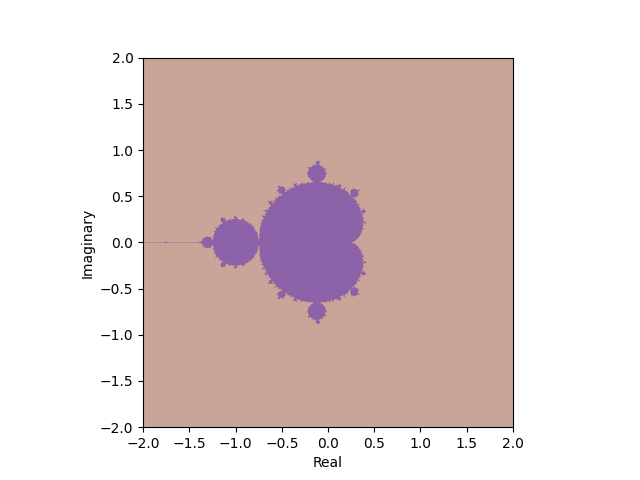
\includegraphics{mandelbrot_2.png}
    \caption{The Mandelbrot set with escaping (orange) and bounded (purple) parameters.}
    \label{fig:mandelbrot_2}
\end{figure}

\lstinputlisting[language=python, caption={Plot the Mandelbrot set (two colors).}, label=lst:mandelbrot_2]{mandelbrot_2.py}

\pagebreak
\hypertarget{3}{%
\section{}\label{3}} Plot the Mandelbrot set $\mathcal{M}$ (many colors)
\begin{enumerate}[label=(\alph{*})]
    \item Plot in color \#0 the set of escaping parameters.
    \item Plot in color \#1 the set of parameters $c_{l,m}$ converging towards a fixed point.
    \item Plot in color \#2 the set of parameters $c_{l,m}$ converging towards a periodic orbit of period two.
    \item Plot in color \#3 the set of parameters $c_{l,m}$ converging towards a periodic orbit of period three.
    \item Plot in color \#4 the set of parameters $c_{l,m}$ converging towards a periodic orbit of period four.
    \item Plot in color \#5 the set of parameters $c_{l,m}$ converging towards a periodic orbit of period five.
\end{enumerate}

With a few modifications on the previous program [Lst.\ref{fig:mandelbrot_2}] we can accomplish the desired result [Lst.\ref{lst:mandelbrot_n}].

\lstinputlisting[
    language=python,
    caption={Plot the Mandelbrot set (many colors).},
    label=lst:mandelbrot_n,
    linerange={50-73}
]{mandelbrot_n.py}
\begin{figure}[ht]
    \centering
    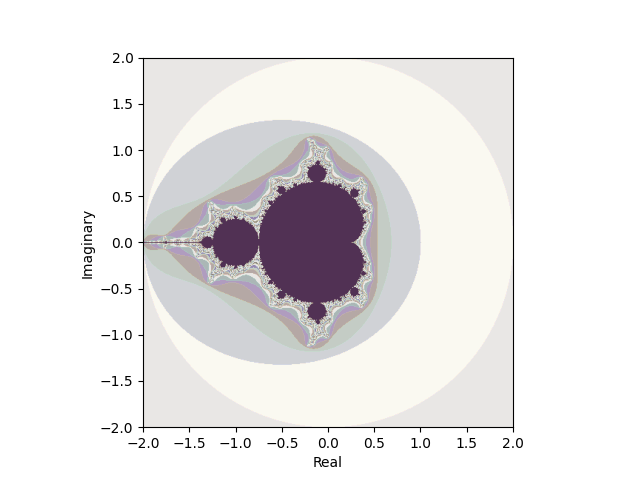
\includegraphics{mandelbrot_n.png}
    \caption{The Mandelbrot set with many colors*.}
    \label{fig:mandelbrot_n}
\end{figure}

\begin{enumerate}[label=(\alph{*})]
    \item The set of escaping parameters is grey.
    \item The set of parameters $c_{l,m}$ converging towards a fixed point is red.
    \item The set of parameters $c_{l,m}$ converging towards a periodic orbit of period two is blue.
    \item The set of parameters $c_{l,m}$ converging towards a periodic orbit of period three is green.
    \item The set of parameters $c_{l,m}$ converging towards a periodic orbit of period four is orange.
    \item The set of parameters $c_{l,m}$ converging towards a periodic orbit of period five is purple.
\end{enumerate}

\textit{* Apologies if the color palette is not soothing, the author is colorblind.}

\newpage
\hypertarget{4}{%
\section{}\label{4}}
A Siegel disk is a Fatou component
where points rotate around an indifferent fixed point. We denote the Golden mean
by $\varphi = \frac{\sqrt{5} - 1}{2} = 0.6180339887...$ and consider the parameter 
$c_{\varphi} = \frac{1}{2}e^{2\pi i \varphi} - \frac{1}{4}e^{4\pi i \varphi}$.

\begin{enumerate}[label=(\alph{*})]
    \item Plot de Dynamical plane of $Q_c(z) = z^2 + c\varphi$. [Fig.\ref{fig:siegel_1}]
    \item Compute the fixed points of $Q_c$ and their multipliers.\\
    To compute the fixed points of the quadratic map $Q_c(z) = z^2 + c{\varphi}$ and their multipliers, we can start by setting $z = Q_c(z)$ and solving for z with the quadratic formula.
    The resulting values of z will be the fixed points and with those we can compute their multipliers by evaluating of $Q_c'(z)$ at each fixed point. The multiplier is given by the absolute value of the derivative [Lst.\ref{lst:fixed}]:
    \lstinputlisting[language=python, caption={Compute the fixed points}, label=lst:fixed]{fixed_points.py}
    Results:
    \begin{lstlisting}
        Fixed point 1 (1.36868443903916+0.3377451471307618j)
        Multiplier 1 2.819481426133763
        Fixed point 2: (-0.36868443903915993-0.3377451471307618j)
        Multiplier 2: 1.0
    \end{lstlisting}
    \item Plot in the dynamical plane the orbit of several (five) points near the indifferent fixed point. [Fig.\ref{fig:siegel_2}]
\end{enumerate}
\pagebreak
\lstinputlisting[language=python, caption={Plot the Dynamical Plane of $Q_c(z) = z^2 + c{\varphi}$ with optional points param.}, label=lst:siegel]{siegel.py}

\newpage
\begin{thebibliography}{X}
\bibitem{chaos}
Dr. Kuennen, Eric.\\
University of Winsconsin-Stout.\\
\textit{GRAPHICAL ANALYSIS, AND ATTRACTING AND REPELLING FIXED POINTS}.\\
\url{http://www.uwosh.edu/faculty_staff/kuennene/Chaos/ChaosNotes2.pdf}.
\end{thebibliography}

\appendix
\section{Figures}

\subsection{Dynamical Plane}
\begin{figure}[ht]
    \centering
    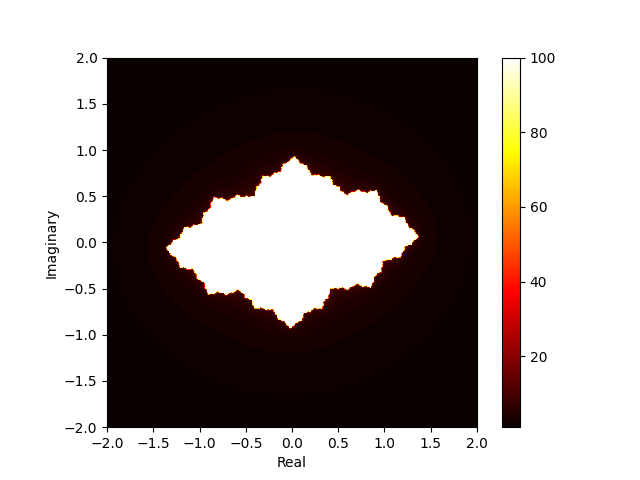
\includegraphics{julia_set_-0.5_0.1.png}
    \caption{Dynamical plane of $c_0$.}
    \label{fig:1a}
\end{figure}
\begin{figure}[ht]
    \centering
    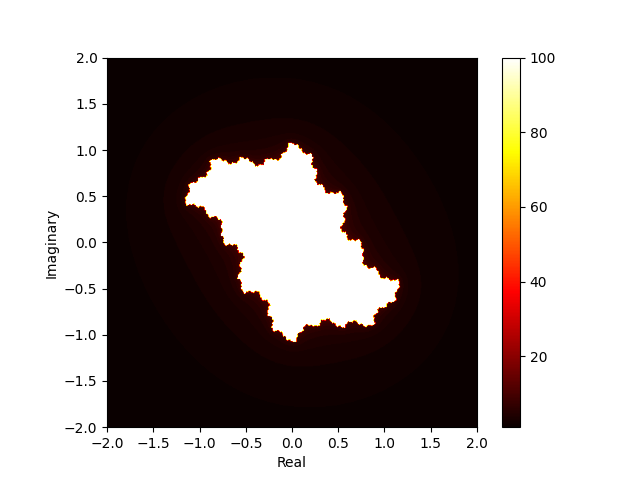
\includegraphics{julia_set_0.0_-0.5.png}
    \caption{Dynamical plane of $c_1$.}
    \label{fig:1b}
\end{figure}
\begin{figure}[ht]
    \centering
    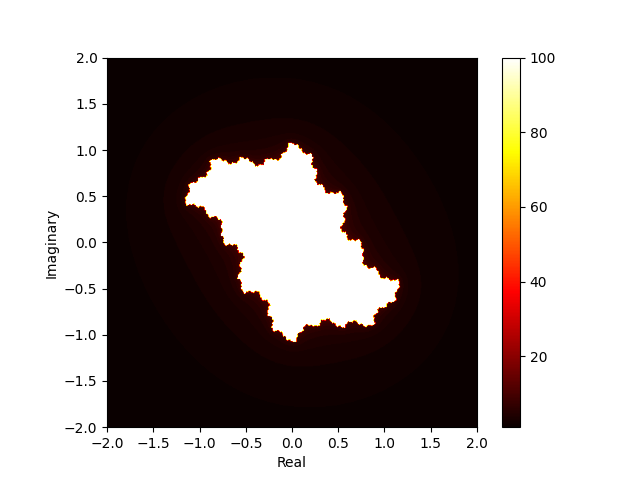
\includegraphics{julia_set_0.0_-0.5.png}
    \caption{Dynamical plane of $c_2$.}
    \label{fig:1c}
\end{figure}
\begin{figure}[ht]
    \centering
    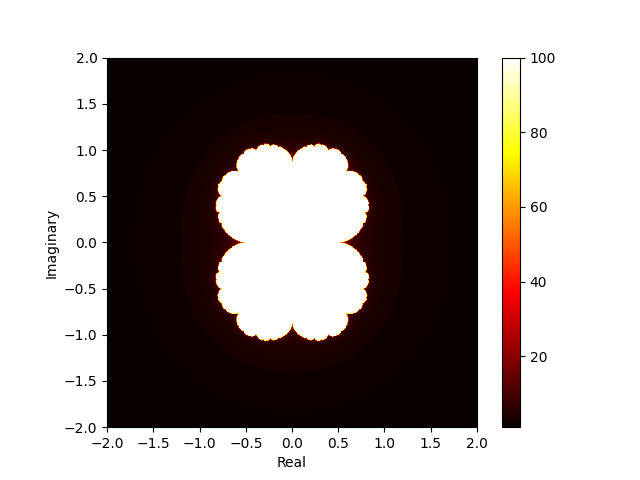
\includegraphics{julia_set_0.25_0.0.png}
    \caption{Dynamical plane of $c_3$.}
    \label{fig:1d}
\end{figure}
\begin{figure}[ht!]
    \centering
    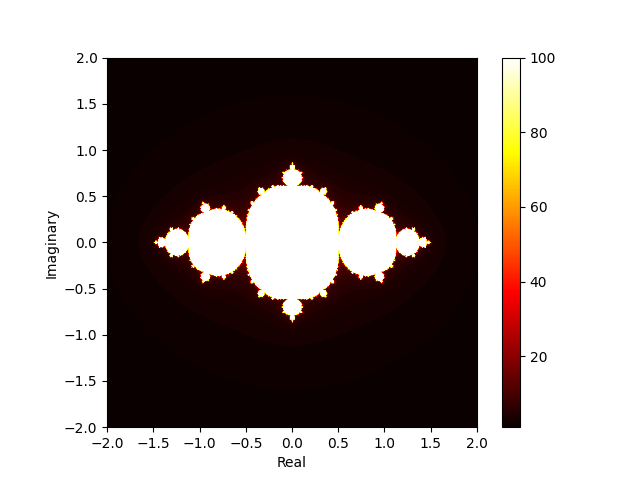
\includegraphics{julia_set_-0.75_0.0.png}
    \caption{Dynamical plane of $c_4$.}
    \label{fig:1e}
\end{figure}

\begin{figure}[ht]
    \centering
    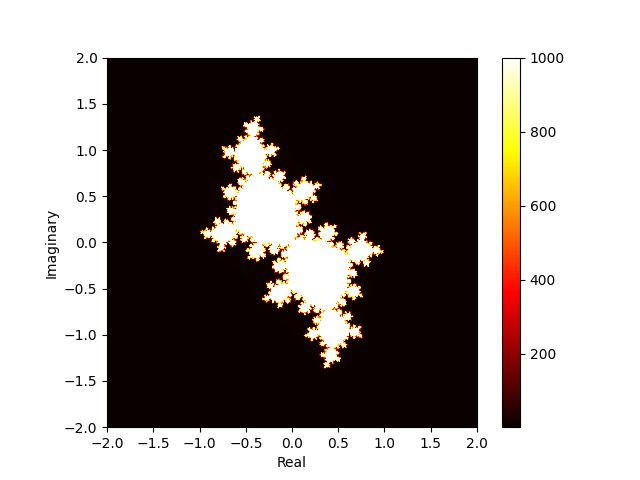
\includegraphics{siegel_1.png}
    \caption{Dynamical plane of $Q_c(z) = z^2 + c_{\varphi}$.}
    \label{fig:siegel_1}
\end{figure}

\begin{figure}[ht]
    \centering
    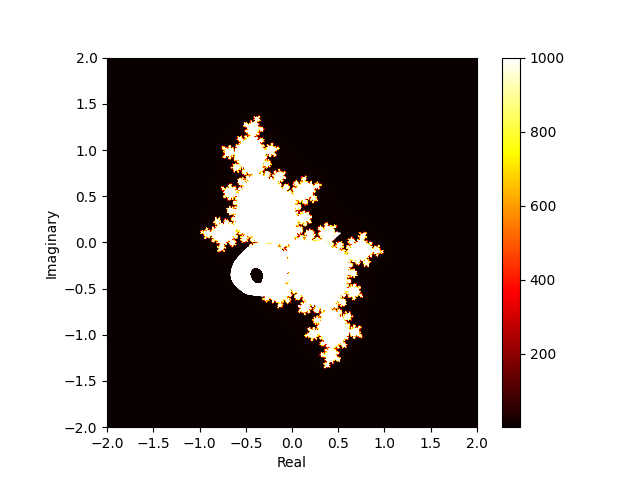
\includegraphics{siegel_2.png}
    \caption{Dynamical plane of $Q_c(z) = z^2 + c_{\varphi}$ with several points near the indifferent fixed point.}
    \label{fig:siegel_2}
\end{figure}

\end{document}
